    \section{Vista de Casos de Uso} \label{vistaCasosDeUso}
    En esta vista se describirá el sistema desde el punto de vista de los casos de uso. El sistema tiene 3 actores:

    \begin{itemize}
        \item \emph{Admin}: administrador de eFuel. Es un usuario de Umbraco, esto es, cuenta con las credenciales para ingresar al back end de Umbraco y, además, tiene los permisos necesarios para administrar las entidades y los miembros de eFuel.
        \item \emph{eFuel Member}: miembro de eFuel, posee credenciales para entrar al sistema.
        \item \emph{Customer}: representa a una o varias estaciones de servicio. Solo tiene acceso a la información referente a las estaciones de servicio asignadas por el administrador del sistema. Es el tipo de miembro que más uso le dará al sistema.
        \item \emph{Staff}: representa a un distribuidor de combustible. Tiene acceso a la información de todas las estaciones de servicio del sistema.
    \end{itemize}

    \subsection{Resumen de Casos de Uso}
    \newcounter{magicrownumbers}
    \newcommand\rownumber{\stepcounter{magicrownumbers}\arabic{magicrownumbers}}
    \begin{center}
        \begin{longtable}{ | l | l | c | }
            \hline
            \rowcolor{gray!30}
            \multicolumn{1}{|c|}{ID del Caso de Uso} &
            \multicolumn{1}{|c|}{Caso de Uso} &
            \multicolumn{1}{|c|}{Actor} \\
            \hhline{===}
            \endhead

            \endfoot

            CU-\rownumber & Iniciar sesión (Umbraco) & Admin \\ \hline
            CU-\rownumber & Consultar lista de miembros & Admin \\ \hline
            CU-\rownumber & Gestionar miembro (CRUD) & Admin \\ \hline
            CU-\rownumber & Asignar cliente/s a miembro & Admin \\ \hline
            CU-\rownumber & Remover cliente/s de miembro & Admin \\ \hline
            CU-\rownumber & Cambiar permisos de miembro & Admin \\ \hline

            CU-\rownumber & Gestionar contenido & Admin \\ \hline
            CU-\rownumber & Consultar lista de clientes & Admin \\ \hline
            CU-\rownumber & Gestionar cliente (CRUD) & Admin \\ \hline
            CU-\rownumber & Consultar lista de productos & Admin \\ \hline
            CU-\rownumber & Gestionar producto (CRUD) & Admin \\ \hline
            CU-\rownumber & Consultar lista de transportes & Admin \\ \hline
            CU-\rownumber & Gestionar transportes (CRUD) & Admin \\ \hline
            CU-\rownumber & Consultar lista de zonas & Admin \\ \hline
            CU-\rownumber & Gestionar zonas (CRUD) & Admin \\ \hline

            CU-\rownumber & Gestionar transacciones & Admin \\ \hline
            CU-\rownumber & Consultar lista de registros & Admin \\ \hline
            CU-\rownumber & Gestionar registro (CRUD) & Admin \\ \hline
            CU-\rownumber & Consultar lista de pedidos & Admin \\ \hline
            CU-\rownumber & Gestionar pedido (CRUD) & Admin \\ \hline
            CU-\rownumber & Consultar lista de detalles de pedidos & Admin \\ \hline
            CU-\rownumber & Gestionar detalle de pedido (CRUD) & Admin \\ \hline
            CU-\rownumber & Consultar lista de facturas & Admin \\ \hline
            CU-\rownumber & Gestionar factura (CRUD) & Admin \\ \hline
            CU-\rownumber & Consultar lista de cobros & Admin \\ \hline
            CU-\rownumber & Gestionar cobro (CRUD) & Admin \\ \hline
            CU-\rownumber & Consultar lista de detalles de cobros & Admin \\ \hline
            CU-\rownumber & Gestionar detalle de cobro (CRUD) & Admin \\ \hline

            CU-\rownumber & Iniciar sesión (eFuel) & Customer, Staff \\ \hline
            CU-\rownumber & Consultar lista de pedidos & Customer, Staff \\ \hline
            CU-\rownumber & Consultar pedido & Customer, Staff \\ \hline
            CU-\rownumber & Filtrar lista de pedidos & Customer, Staff \\ \hline
            CU-\rownumber & Exportar lista de pedidos & Customer, Staff \\ \hline
            CU-\rownumber & Crear pedido & Customer, Staff \\ \hline
            CU-\rownumber & Seleccionar cliente & Customer, Staff \\ \hline
            CU-\rownumber & Seleccionar fecha & Customer, Staff \\ \hline
            CU-\rownumber & Seleccionar turno  & Customer, Staff \\ \hline
            CU-\rownumber & Seleccionar transporte  & Customer, Staff \\ \hline
            CU-\rownumber & Seleccionar productos & Customer, Staff \\ \hline

            CU-\rownumber & Consultar lista de facturas & Customer, Staff \\ \hline

            CU-\rownumber & Consultar lista de clientes & Customer, Staff \\ \hline
            CU-\rownumber & Consultar cliente & Customer, Staff \\ \hline
            CU-\rownumber & Consultar pedidos de cliente & Customer, Staff \\ \hline

            CU-\rownumber & Consultar lista de transportes & Customer, Staff \\ \hline

            CU-\rownumber & Importar lista de transportes & Customer, Staff \\ \hline

            CU-\rownumber & Consultar lista de zonas & Customer, Staff \\ \hline

            CU-\rownumber & Importar lista de zonas & Customer, Staff \\ \hline

        \end{longtable}
    \end{center}

    \subsection{Diagrama de Casos de Uso}
    Se separaron los casos de uso en varios diagramas para facilitar la lectura.

    \begin{figure}[H]
        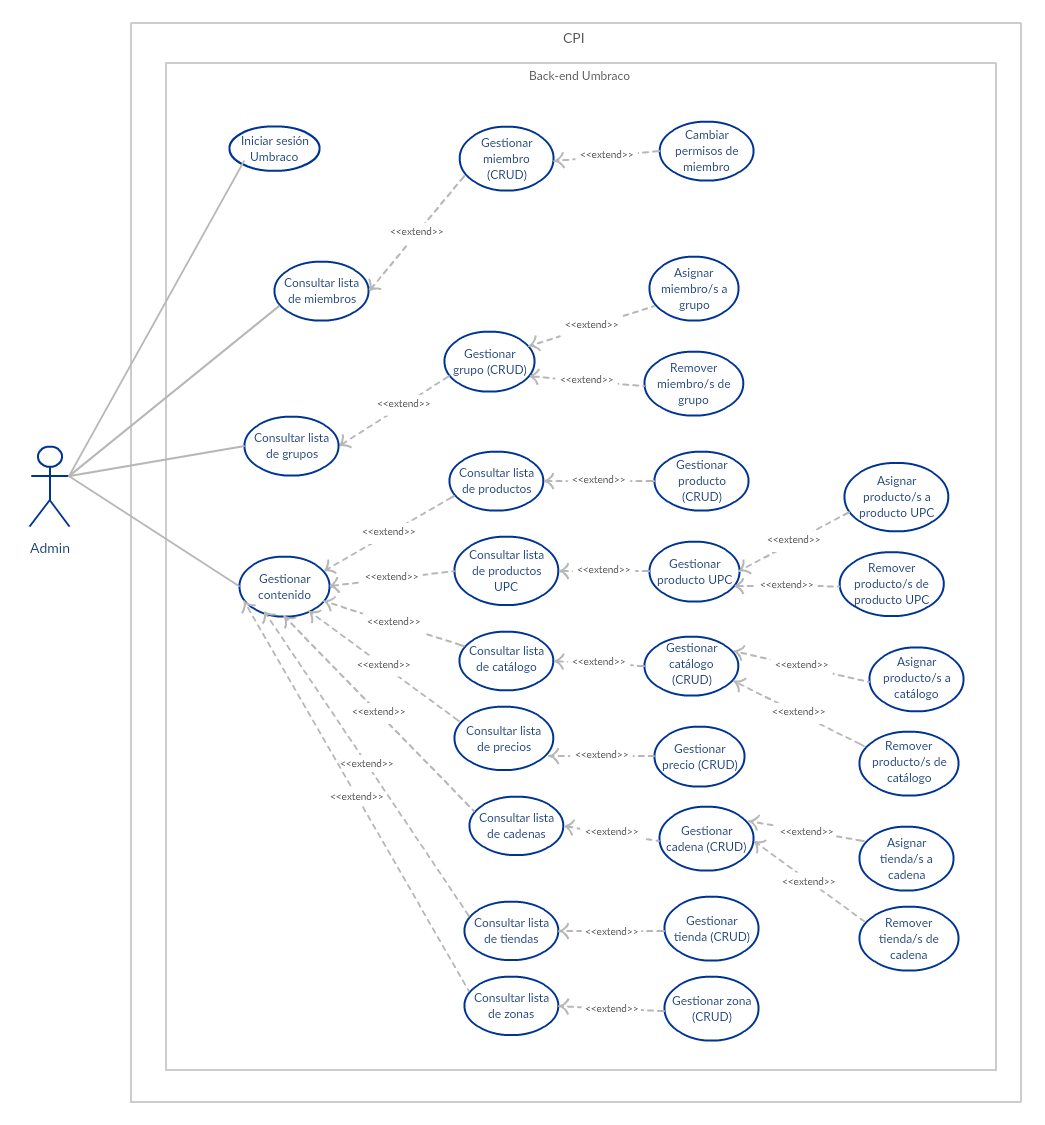
\includegraphics[width=\textwidth]{cu_admin.png}
        \centering
    \end{figure}

    \begin{figure}[H]
        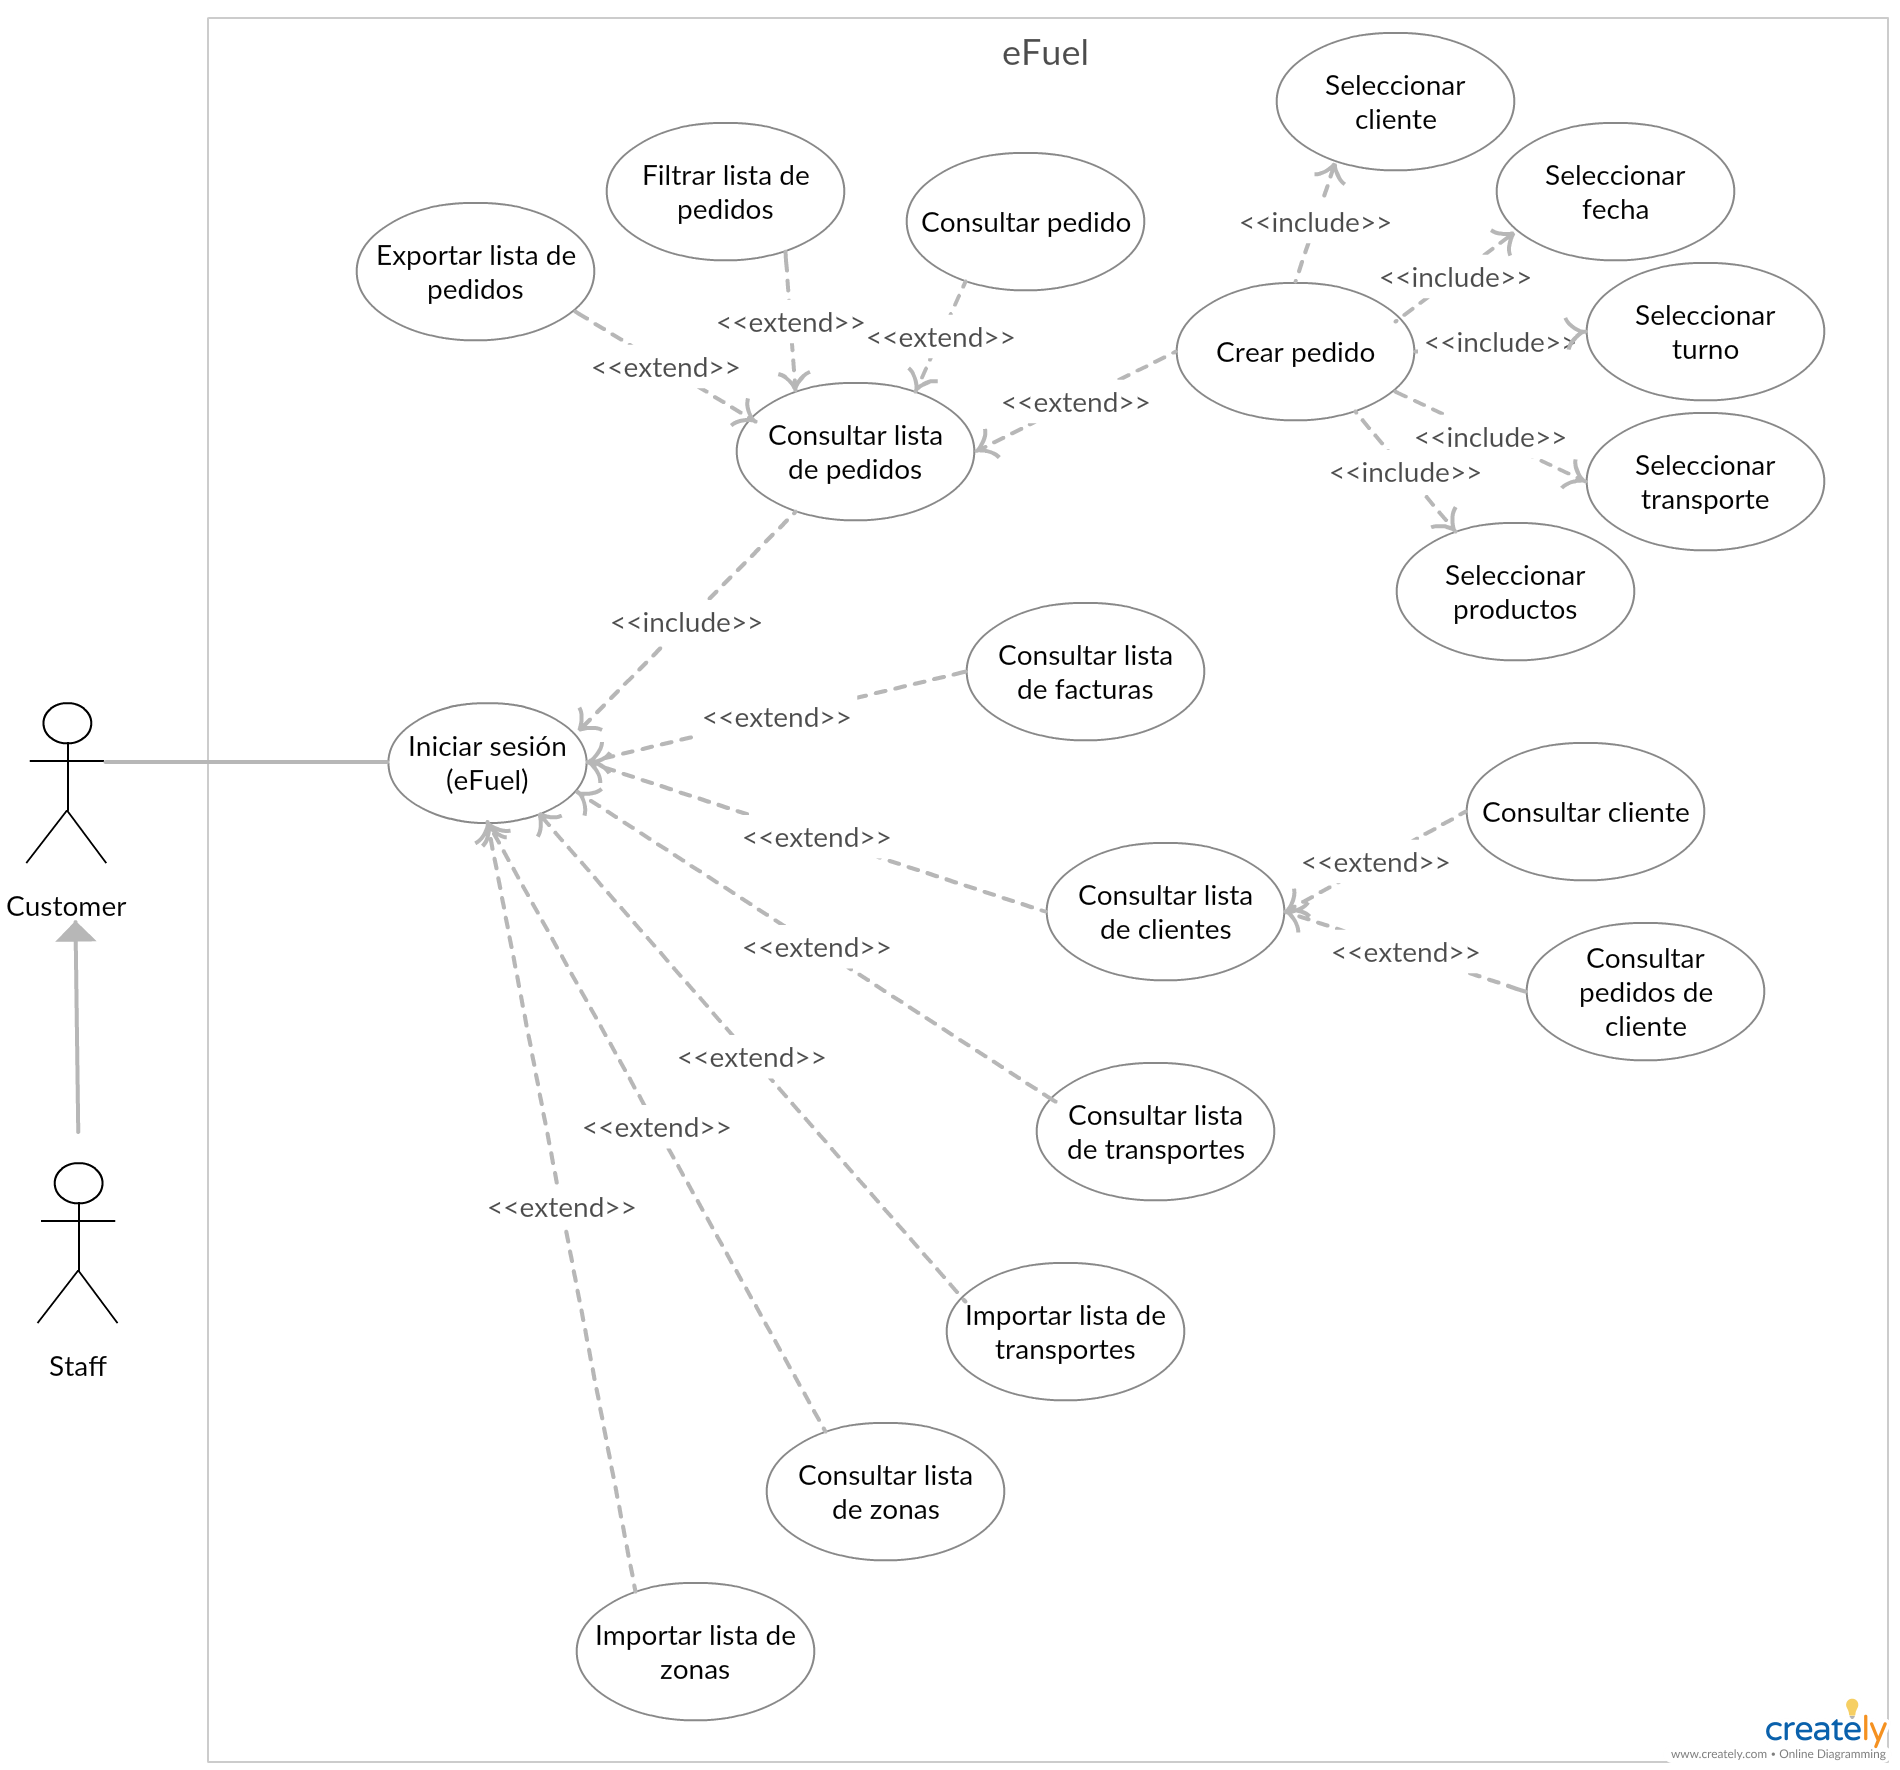
\includegraphics[width=\textwidth]{cu_customer_staff.png}
        \centering
    \end{figure}

    \subsection{Especificaciones de Casos de Uso}
    A continuación las narrativas de los casos de uso:

    \begin{center}
        \begin{longtabu} to 0.9\textwidth { | X[p] | X[p] | }
            \hline
            \multicolumn{2}{|l|}{
                \cellcolor{gray!30}{\large{\textbf{Caso de Uso:}} Iniciar sesión (Umbraco)}
            } \TBstrut \\
            \hline\hline

            \multicolumn{2}{|l|}{
                \makecell{\large{\textbf{Descripción:}} \\ El usuario quiere ingresar al back end de Umbraco.}
            } \\
            \hline

            \multicolumn{2}{|l|}{
                \makecell{\large{\textbf{Precondición:}} \\ Haber ingresado la dirección correcta del sitio en la barra de navegación.}
            } \\
            \hline


            \multicolumn{2}{|l|}{\cellcolor{gray!15}\large{\textbf{Flujo básico:}}}  \TBstrut\\
            \hline

            Actor & Sistema \TBstrut\\
            \hline
            1. El actor abre su navegador e introduce la dirección correspondiente al back end de Umbraco. &  \\ [0.3ex]
            \hline
             & 2. El servidor procesa la solicitud y envía al navegador del cliente una ventana para que el usuario se autentique. \\ [0.3ex]
             \hline
             3. El actor introduce su email y su contraseña. &  \\ [0.3ex]
             \hline
             & 4. El sistema valida la información del usuario y lo redirige al tablero (back end) de Umbraco. \\ [0.3ex]
             \hline\hline


            \multicolumn{2}{|l|}{\cellcolor{gray!15}\large{\textbf{Flujos alternos:}}}  \TBstrut\\
            \hline

            Actor & Sistema \TBstrut\\
            \hline
            1. El actor abre su navegador e introduce la dirección correspondiente al back end de Umbraco. &  \\ [0.3ex]
            \hline
             & 2. El servidor procesa la solicitud y envía al navegador del cliente una ventana para que el usuario se autentique. \\ [0.3ex]
             \hline
             3. El actor introduce su email y su contraseña. &  \\ [0.3ex]
             \hline
             & 4. El sistema no valida la información del usuario y lo redirige a la misma página de inicio de sesión indicándole que los datos introducidos son incorrectos. \\ [0.3ex]
             \hline\hline

            \multicolumn{2}{|l|}{
                \makecell{\large{\textbf{Poscondición:}} \\ El usuario se encuentra en el tablero de Umbraco.}
            } \\
            \hline
            \multicolumn{2}{|l|}{
                \makecell{\large{\textbf{Puntos de extensión:}} \\ No se requiere de otros casos de uso.}
            } \\
            \hline
        \end{longtabu}
    \end{center}
    \vspace{-4em}

    \begin{center}
        \begin{longtabu} to 0.9\textwidth { | X[p] | X[p] | }
            \hline
            \multicolumn{2}{|l|}{
                \cellcolor{gray!30}{\large{\textbf{Caso de Uso:}} Consultar lista de miembros}
            } \TBstrut \\
            \hline\hline
            \multicolumn{2}{|l|}{
                \makecell{\large{\textbf{Descripción:}} \\ El usuario quiere consultar la lista de miembros de eFuel.}
            } \\
            \hline
            \multicolumn{2}{|l|}{
                \makecell{\large{\textbf{Precondición:}} \\ Haber ingresado al back end de Umbraco.}
            } \\
            \hline
            \multicolumn{2}{|l|}{\cellcolor{gray!15}\large{\textbf{Flujo básico:}}}  \TBstrut\\
            \hline

            Actor & Sistema \TBstrut\\
            \hline
            1. El usuario le da click a la sección "Members" en el tablero de Umbraco. &  \TBstrut\\
            \hline
            & 2. El sistema muestra el panel de miembros. \TBstrut\\
            \hline
            3. El usuario le da click a la carpeta "Members" y selecciona "eFuel Member". &  \TBstrut\\
            \hline
            & 4. El sistema muestra la lista de los miembros de eFuel. \TBstrut\\
            \hline\hline


            \multicolumn{2}{|l|}{\cellcolor{gray!15}\large{\textbf{Flujos alternos:}}}  \TBstrut\\
            \hline
            Actor & Sistema \TBstrut\\
            \hline
            1. El actor hace algo. &  \TBstrut\\
            \hline
             & 2. El sistema responde. \TBstrut\\
             \hline\hline


            \multicolumn{2}{|l|}{
                \makecell{\large{\textbf{Poscondición:}} \\ Aquí va la poscondición del caso de uso.}
            } \\
            \hline
            \multicolumn{2}{|l|}{
                \makecell{\large{\textbf{Puntos de extensión:}} \\ Aquí van los puntos de extensión del caso de uso.}
            } \\
            \hline
        \end{longtabu}
    \end{center}
    \vspace{-4em}

    \begin{center}
        \begin{longtabu} to 0.9\textwidth { | X[p] | X[p] | }
            \hline
            \multicolumn{2}{|l|}{
                \cellcolor{gray!30}{\large{\textbf{Caso de Uso:}} Nombre del caso de uso}
            } \TBstrut \\
            \hline\hline
            \multicolumn{2}{|l|}{
                \makecell{\large{\textbf{Descripción:}} \\ Descripción del caso de uso.}
            } \\
            \hline
            \multicolumn{2}{|l|}{
                \makecell{\large{\textbf{Precondición:}} \\ Aquí va la precondición.}
            } \\
            \hline
            \multicolumn{2}{|l|}{\cellcolor{gray!15}\large{\textbf{Flujo básico:}}}  \TBstrut\\
            \hline

            Actor & Sistema \TBstrut\\
            \hline
            1. El actor hace algo. &  \TBstrut\\
            \hline
             & 2. El sistema responde. \TBstrut\\
             \hline\hline


            \multicolumn{2}{|l|}{\cellcolor{gray!15}\large{\textbf{Flujos alternos:}}}  \TBstrut\\
            \hline
            Actor & Sistema \TBstrut\\
            \hline
            1. El actor hace algo. &  \TBstrut\\
            \hline
             & 2. El sistema responde. \TBstrut\\
             \hline\hline


            \multicolumn{2}{|l|}{
                \makecell{\large{\textbf{Poscondición:}} \\ Aquí va la poscondición del caso de uso.}
            } \\
            \hline
            \multicolumn{2}{|l|}{
                \makecell{\large{\textbf{Puntos de extensión:}} \\ Aquí van los puntos de extensión del caso de uso.}
            } \\
            \hline
        \end{longtabu}
    \end{center}
    \vspace{-4em}